\chapter{Bandwidth Efficient Pilot-based CSI Feedback}
\label{chap:p2d}

This chapter details an estimator for the UE-side angular-delay domain CSI based on a limited number of spatial-frequency domain pilots. This scheme adheres to the 3GPP standards for pilot allocation across time-frequency resources as described in Section~\ref{sect:pilots}.

Section~\ref{sect:p2de} details our proposed pilots-to-delay estimator (P2DE), and Figure~\ref{fig:p2d} demonstrates the operating principle behind P2DE. Appendix~\ref{appdx:odir} describes off-diagonal regularization as a countermeasure for ill-conditioned CSI matrices. Section~\ref{sect:diag} explicitly links the proposed P2DE to the 3GPP placement of CSI-RS/DMRS resource elements and describes our proposed diagonal pilot pattern which adheres to LTE/NR specifications. Section~\ref{sect:hetero-markov} describes an extension of our previously proposed differential encoding network which uses heterogeneous CNNs for different timeslots. Finally, Section~\ref{sect:p2de-results} presents results for the P2DE and our propose heterogeneous differential encoding networks.

\begin{figure}[!hbtp]
    \centering
    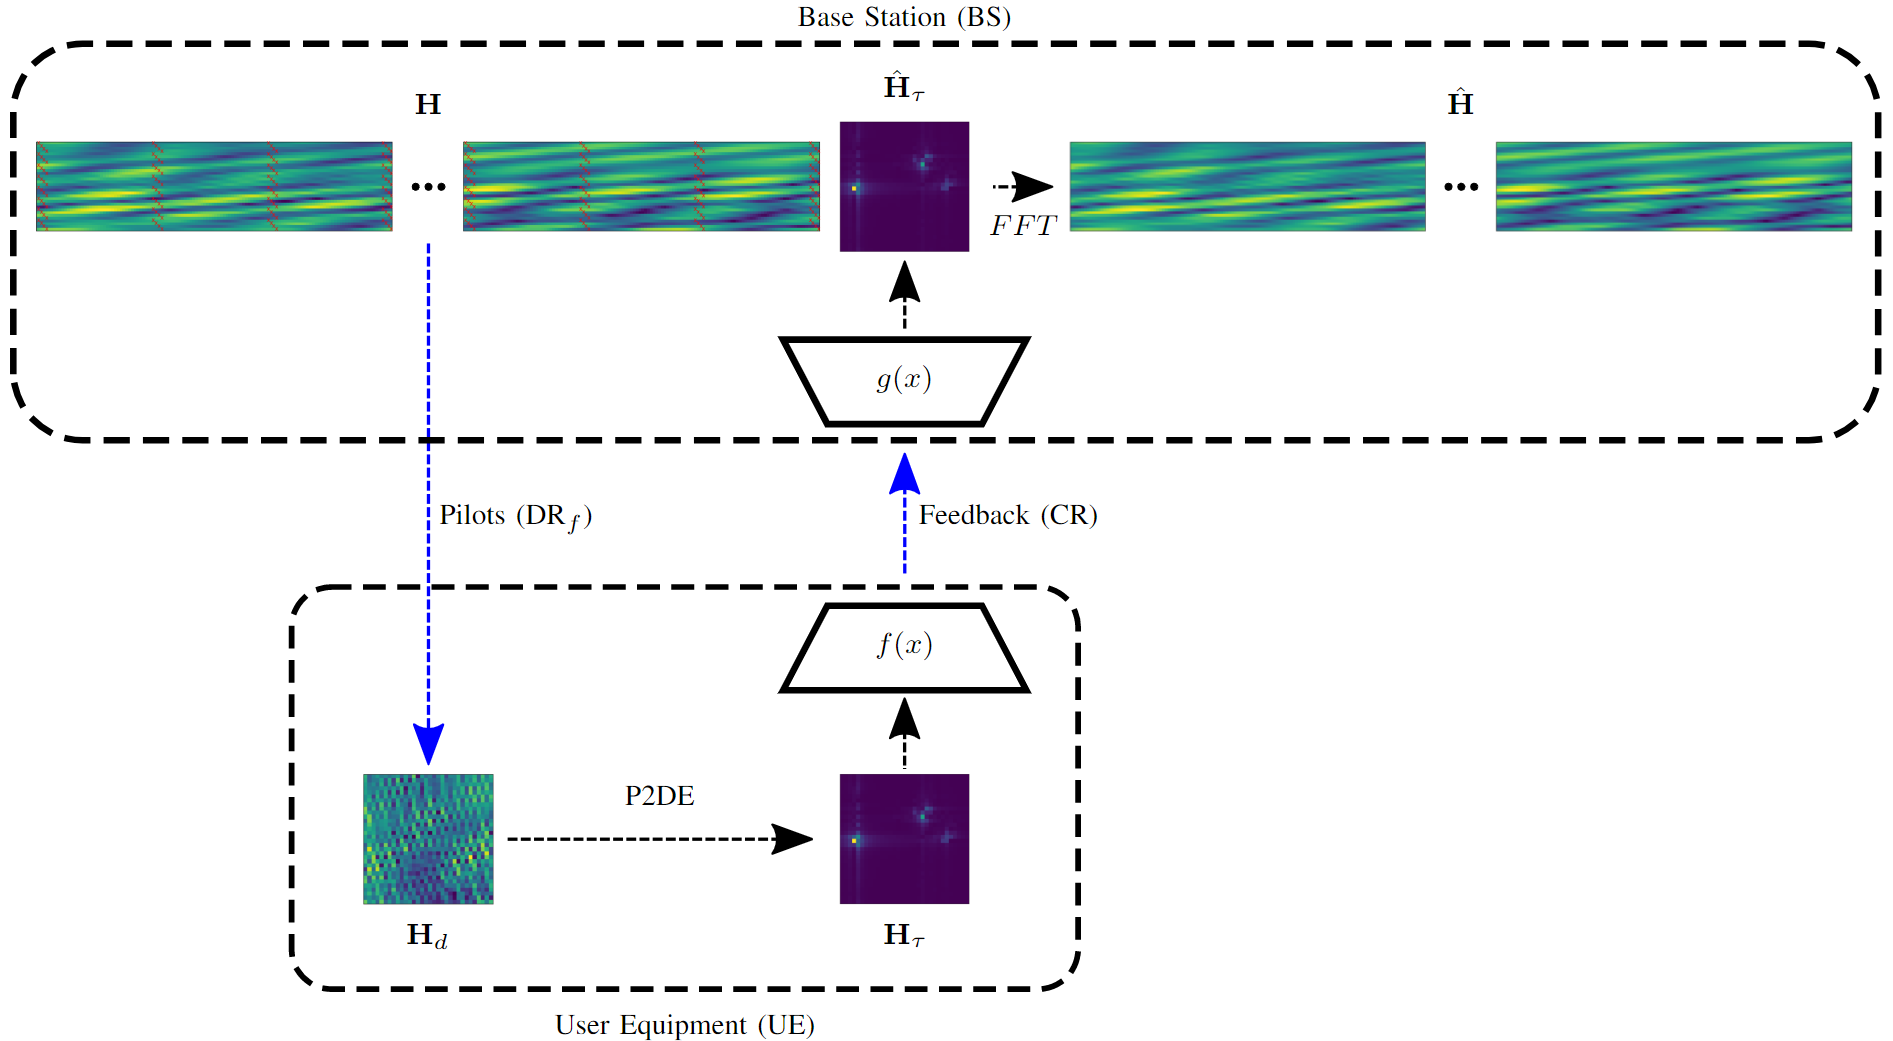
\includegraphics[width=\linewidth]{./images/00_downlink_p2d_feedback_horiz_diag.png}
    \caption{Compressive CSI estimation based on linear P2D estimator. First,
    we use downlink pilots to 
    generate a sparse, frequency domain CSI
    estimate 
    of size $M_f << N_f$. We then apply
    the P2D estimator, $\mathbf{Q}^\dag_{N_t}$ of (\ref{eq:p2d_short}), to establish 
    the truncated
    delay domain CSI estimate.
    We train a
    learnable encoder, 
    $f(x)$,
    and decoder, $g(x)$, to compress and decode the feedback, respectively. The 
    gNB recovers
    the frequency domain
    CSI from 
    the decoded 
    delay domain CSI estimate.}
    \label{fig:p2d}
\end{figure}

\section{Pilots-to-delay Estimator (P2DE)}
\label{sect:p2de}

Denote $\boldeta_i \in \mathbb{C}^{N_f}$ as the $i$-th row of the spatial-frequency matrix $\mathbf{H}$, and denote the downsampled version of $\boldeta_i$ as $\boldeta_{d,i} \in \mathbb{C}^{M_f}$ where $M_f << N_f$. Thus, the spatial-frequency CSI, $\mathbf{H}$, and its downsampled counterpart, $\mathbf{H}_d$, can be written as,
\begin{equation}
	\mathbf{H} = \begin{bmatrix} \boldeta_1 \\ \boldeta_2 \\ \vdots \\ \boldeta_{N_b} \\\end{bmatrix}\in\mathbb{C}^{N_b \times N_f}, \; \mathbf{H}_d = \begin{bmatrix} \boldeta_{d,1} \\ \boldeta_{d,2} \\ \vdots \\ \boldeta_{d,N_b} \\\end{bmatrix}\in\mathbb{C}^{N_b \times M_f}.
\end{equation}
$\boldeta_{d,i}$ is related to $\boldeta_i$ by the downsampling matrix for the $i$-th antenna port, $\mathbf{P}_i$, as
\begin{equation}
	\boldeta_{d,i} = \boldeta_i \mathbf{P}_i \; \forall \; i \in [1, \dots, N_b].
\end{equation}
Denote the delay-domain CSI vector, $\tilde{\boldeta}_i$, which is defined as
\begin{equation}
	\tilde{\boldeta}_{i}\mathbf{F} = \boldeta_i, \label{eq:dft}
\end{equation}
where $\mathbf{F}$ is the $\mathbf{C}^{N_f \times N_f}$ discrete Fourier transform (DFT) matrix. To relate the frequency domain pilots to the delay domain, we apply the pilot downsampling matrix $\mathbf{P}_i$ to both sides of (\ref{eq:dft}),
\begin{align}
	\tilde{\boldeta}_{i}\mathbf{F}\mathbf{P}_i = \boldeta_i\mathbf{P}_i \nonumber \\
	\tilde{\boldeta}_{i}\mathbf{Q}_i = \boldeta_{d,i} \label{eq:qmat}
\end{align}
where $\mathbf{Q}_i=\mathbf{F}\mathbf{P}_i\in\mathbb{C}^{N_f\times M_f}$ is the downsampled DFT matrix.
Leveraging the sparsity of CSI data in the delay domain (see Section~\ref{sect:sparse-csi}, Figure~\ref{fig:freq-vs-delay}), many works choose to feedback and compress the truncated delay domain vectors, $\tilde{\boldeta}_{c,i}\in\mathbb{C}^{N_t}$. The zero-padded vector $\tilde{\boldeta}_{i}$ defined as
\begin{align} 
	\tilde{\boldeta}_{i} = \left[\tilde{\boldeta}_{c,i}, \mathbf{0}_{N_f - N_t}\right]. \label{eq:p2d_short}
\end{align}

Based on \ref{eq:qmat}, the delay domain can be related directly to the pilots by taking the pseudoinverse,
\begin{align}
	\tilde{\boldeta}_{i}\mathbf{Q}_i\mathbf{Q}_i^T &= \boldeta_{d,i}\mathbf{Q}_i^T \nonumber \\
	\tilde{\boldeta}_{i} &= \boldeta_{d,i}\mathbf{Q}_i^T\left(\mathbf{Q}_i\mathbf{Q}_i^T\right)^{-1} \nonumber \\
	&= \boldeta_{d,i}\mathbf{Q}_i^{\#} \label{eq:p2d}
\end{align}

% \subsection{Regularization of P2DE} \label{sect:odir}

When the pilot patterns $\mathbf{P}_i$ are equidistant and regularly spaced, the P2DE matrices $\mathbf{Q}_i\mathbf{Q}_i^T$ are typically well-conditioned. However, more irregular patterns can result in ill-conditioned matrices $\mathbf{Q}_i\mathbf{Q}_i^T$, making these matrix inversions unstable. To compensate for this ill-conditioning, we propose to use off-diagonal regularization (ODIR) to condition the P2DE matrices. This form of regularization is described in more detail in Appendix~\ref{appdx:odir}. 

\begin{figure}[!hbtp]
    \centering
    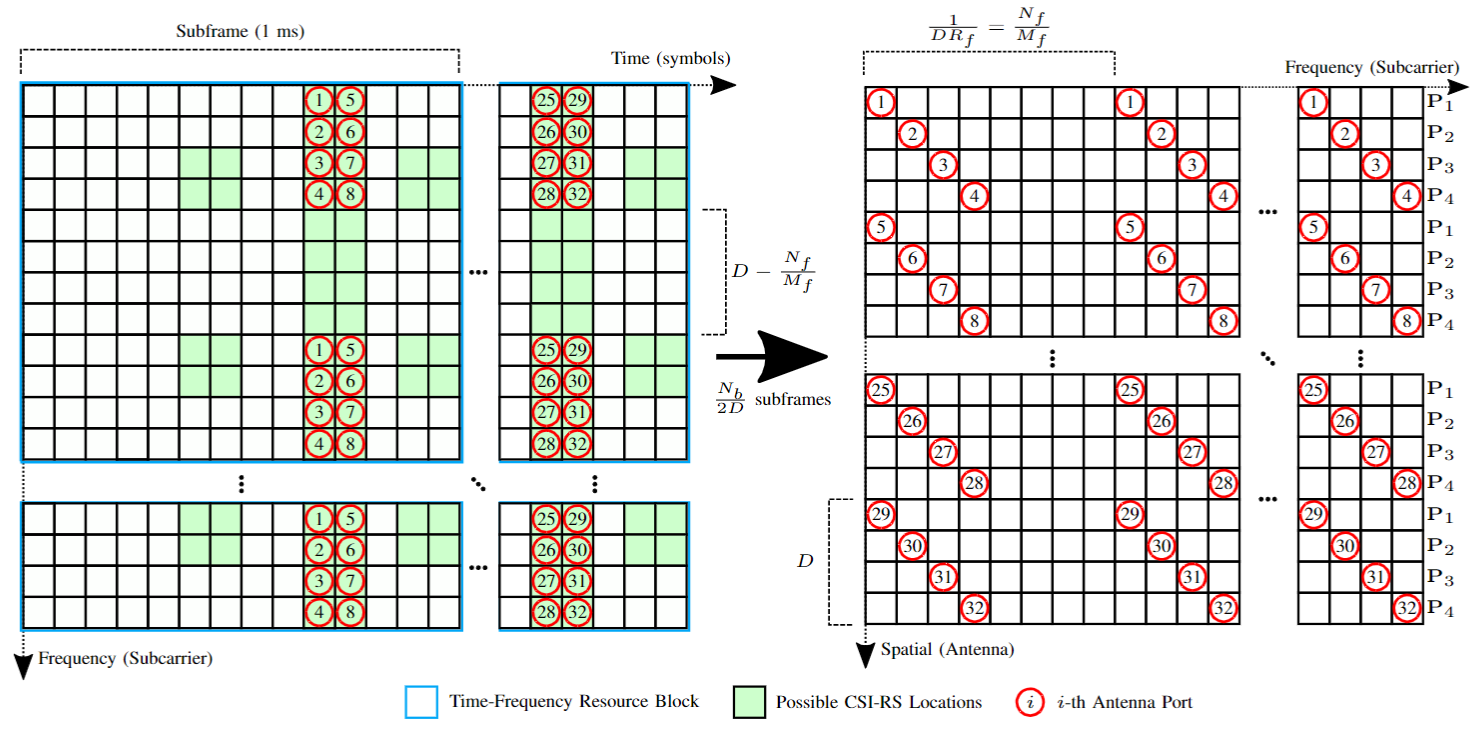
\includegraphics[width=\linewidth]{images/01_p2d_pilots_diag_with_resource_grid.png}
    \caption{(a) LTE Resource Blocks and CSI-RS locations where antenna port pilots are allocated. (b) Schematic for diagonal pilots with relevant parameters, size of diagonal $D$ and frequency downsampling ratio $\text{DR}_f$. In this diagram, $N_b=32, D=4, \text{DR}_f=\frac 18$. The pilot matrix $\mathbf{P}_j$ indicates the downsampling pattern for the $j$-th element of the diagonal pattern. The number of subframes necessary to populate (b) is inversely proportional to $D$.}
    \label{fig:p2d_diag}
\end{figure}

\subsection{Diagonal Pilot Allocations for 3GPP Standards} \label{sect:diag}

As discussed in Section~\ref{sect:pilots}, 3GPP specifications describe the allocation of pilots to time-frequency resources in 4G/LTE \cite{ref:3gpp.36.211, ref:Asplund2020} and 5G/NR \cite{ref:3GPPTS38.211V15.8.0} radio networks, where the reserved resource elements are called CSI reference signals (CSI-RS) for the former and demodulation reference signals (DMRS) for the latter.

In order to connect the P2DE as described in Section~\ref{sect:p2de} to the 3GPP specifications, we must specify the corresponding pilot patterns in the time-frequency grid. In Figure~\ref{fig:p2d_diag}, we show an example of our proposed `diagonal' pilot pattern in an LTE network using CSI-RS locations. We refer to this pattern as diagonal since it is diagonal in the spatial-frequency domain. The benefit of the diagonal pattern can be understood by considering the time needed to acquire downsampled CSI matrix, $\mathbf{H}_d$.

\begin{figure}[!hbtp]
    \centering
    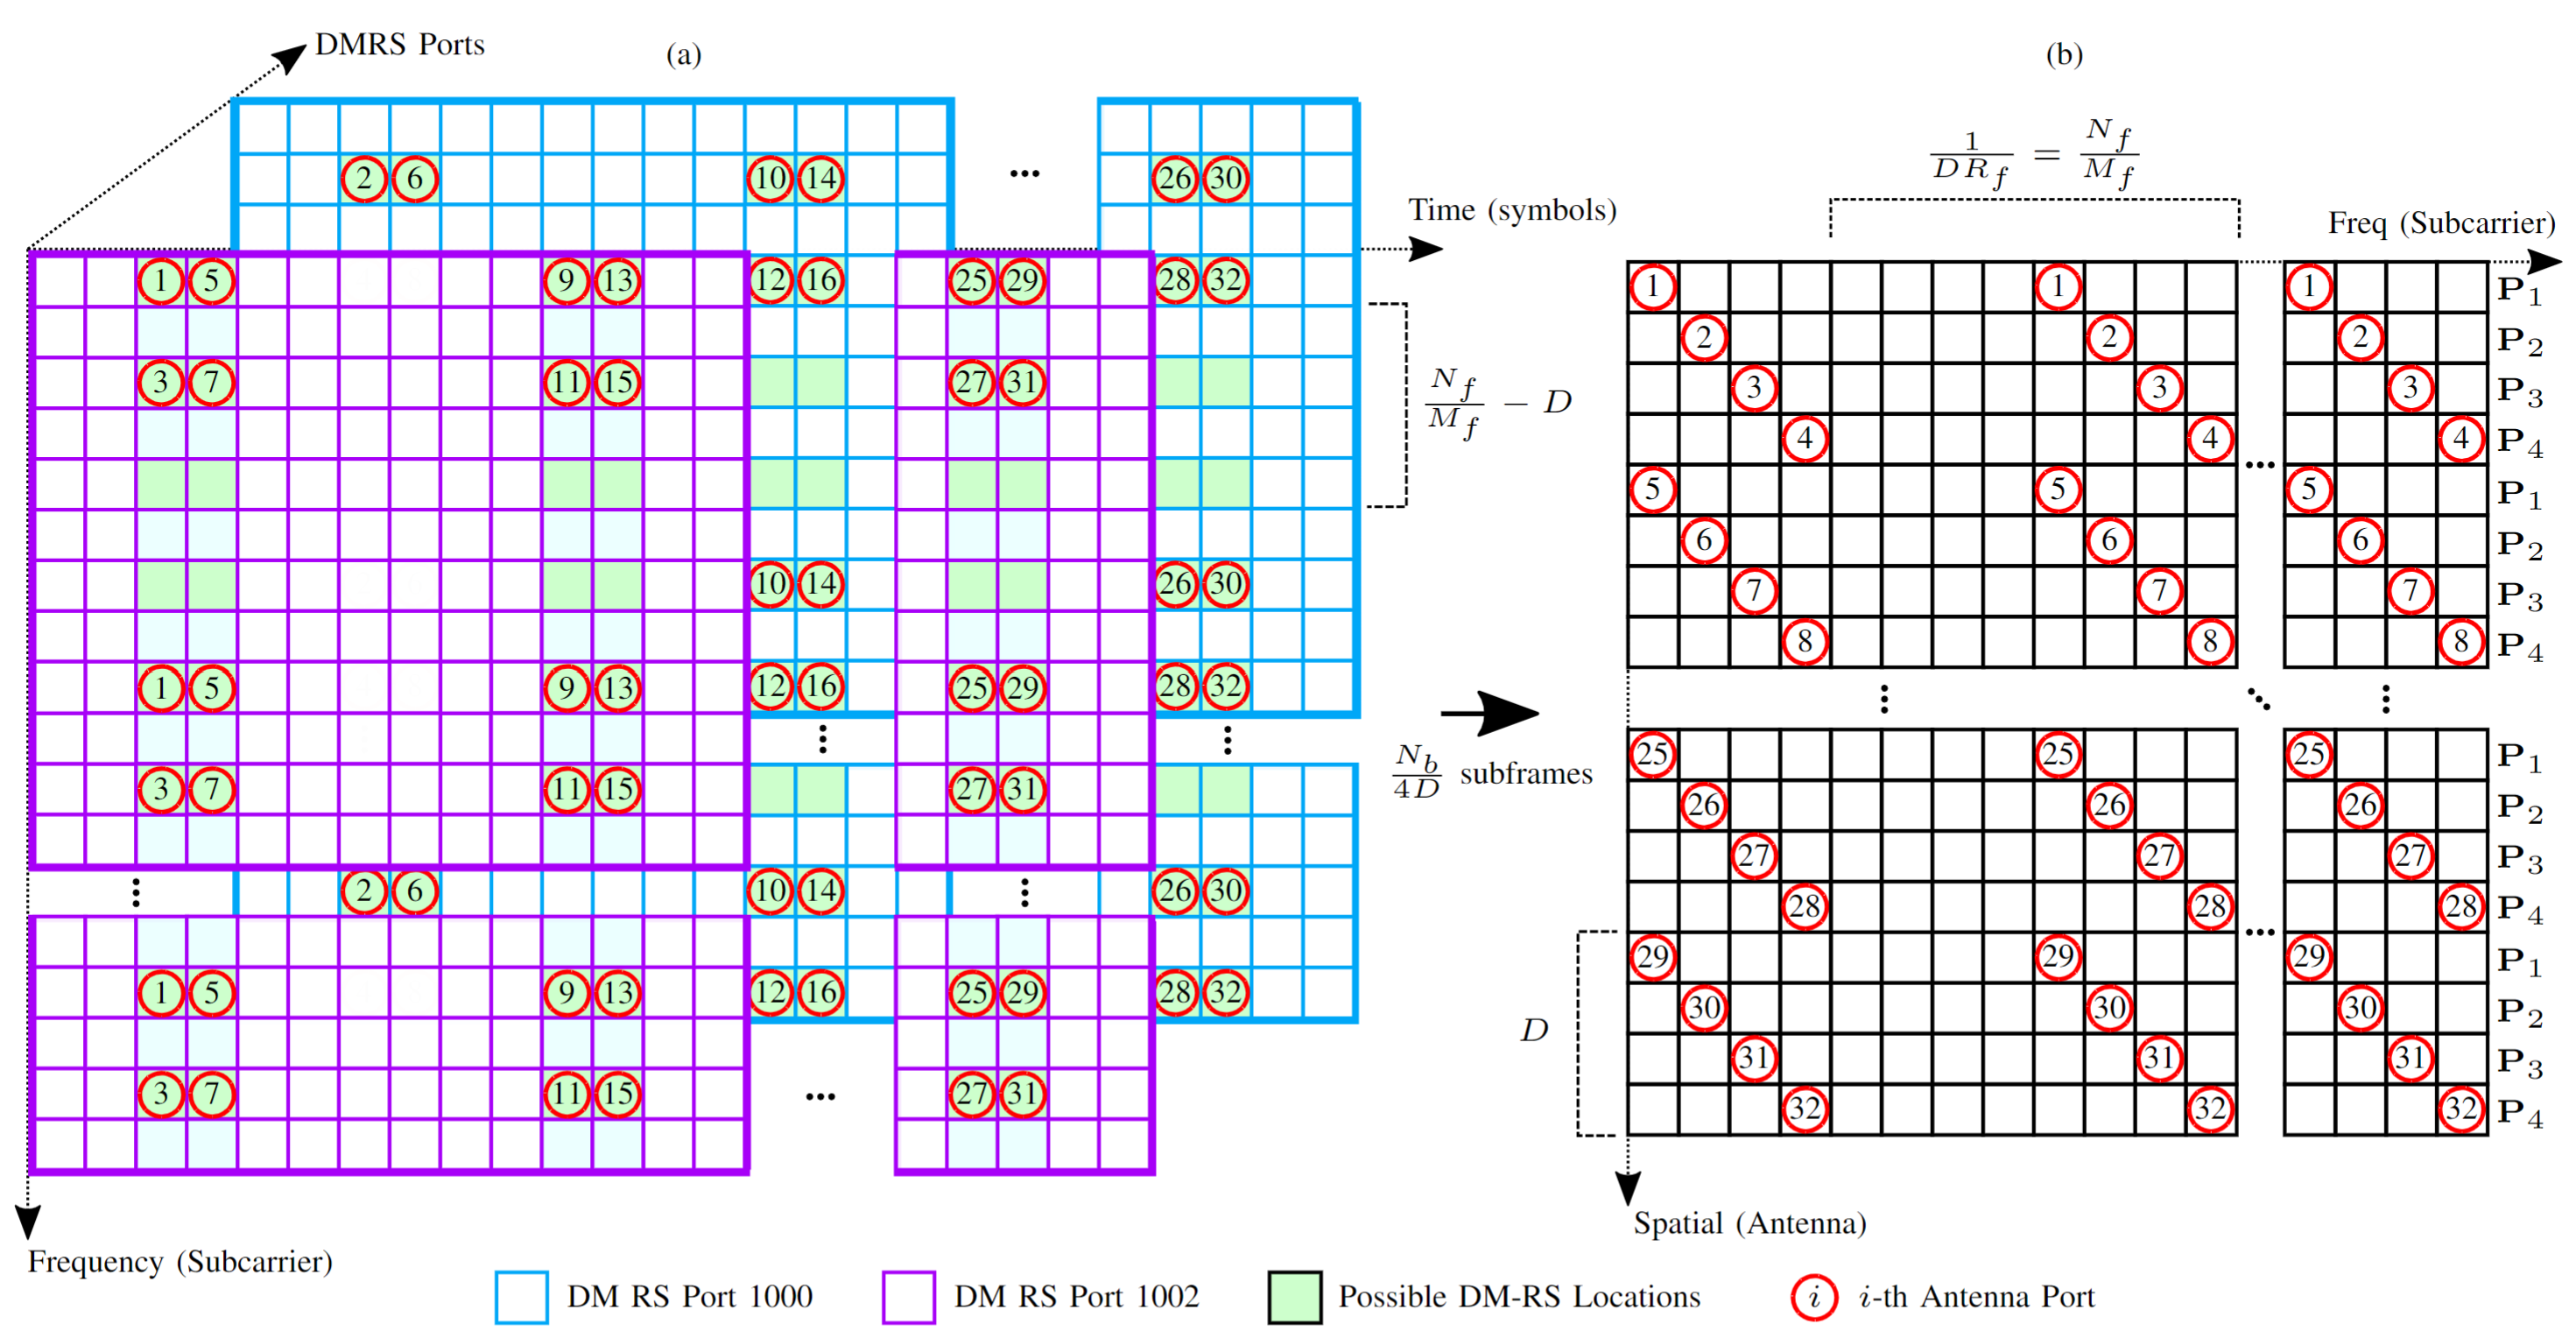
\includegraphics[width=\linewidth]{images/03_p2d_pilots_diag_with_resource_grid_5gnr_ortho.png}
    \caption{(a) 5G NR Resource Blocks and DMRS locations where antenna port pilots are allocated. (b) Schematic for diagonal pilots with relevant parameters, size of diagonal $D$ and frequency downsampling ratio $\text{DR}_f$. In this diagram, $N_b=32, D=4, \text{DR}_f=\frac 18$. The pilot matrix $\mathbf{P}_j$ indicates the downsampling pattern for the $j$-th element of the diagonal pattern. The number of subframes necessary to populate (b) is inversely proportional to $D$.}
    \label{fig:p2d_diag_5gnr}
\end{figure}

Algorithm~\ref{alg:p2d-diag} shows the process for acquiring the delay domain P2DE from sparse frequency domain pilots.

\begin{algorithm}
    \caption{Pilots-to-delay Estimator (P2D) for Diagonal Pilot Pattern} 
    \label{alg:p2d-diag}
    \begin{algorithmic}[1]
    \State \textbf{\emph{Input}}:
        P2DE Matrices, $\mathbf{Q}_{c,j}^\#,\;
        j\in\{1,\dots, D\}$
    \State \textbf{\emph{Input}}: Pilot spatial-frequency CSI, $\mathbf{H}_d\in\mathbb{C}^{N_b\times M_f}$
    \State \textbf{\emph{Initialize}}: Spatial-delay CSI, $\tilde{\mathbf{H}}_\tau\in\mathbb{C}^{N_b\times N_t}$
   \State \textbf{\emph{Initialize}}: Angular-delay CSI estimate, ${\mathbf{H}}_\tau
              \in\mathbb{C}^{N_b\times N_t}$
   \For {$i=1,2,\ldots, N_b$}
        \State \textbf{\# \emph{Index for $j$-th pilot matrix}}
        \State $j = ((i-1) \text{ mod } D) + 1$
        \State \textbf{\# \emph{Apply P2D to $i$-th antenna port}}
        \State ${\boldeta}_{d,i} = \mathbf{H}_d(i,:)$
        \State $\tilde{{\mathbf{H}}}_{\tau}(i,:) = {\boldeta}_{d,i}\mathbf{Q}^{\#}_{c,j}$
        \EndFor
        \State \textbf{\# \emph{Convert from spatial to angular}}
        \State ${{\mathbf{H}}}_{\tau}=\mathbf{F}_{N_b}\tilde{{\mathbf{H}}}_{\tau}$
        \State \textbf{\emph{Return}} ${{\mathbf{H}}}_{\tau}$
    \end{algorithmic} 
\end{algorithm}

\section{Heterogeneous Differential Encoding with P2DE}
\label{sect:hetero-markov}

Chapter~\ref{chap:markovnet} introduced the concept of differential encoding for CSI feedback compression. The delay domain P2DE CSI introduced in this chapter can also be used in the differential encoding framework. Figure~\ref{fig:markov-p2d} showcases the data path when utilizing the P2D estimates with a differential encoding network.

The prior work proposed a differential encoding network that used an identical autoencoder at each timeslot. We refer to such a network as `homogeneous.' In contrast, we can consider a `heterogeneous' network, where we use different network architectures at different timeslots.

In this section, we describe a heterogeneous differential encoder which combines deep compressive sensing with deep autoencoders.

\begin{figure}[!hbtp]
    \centering
    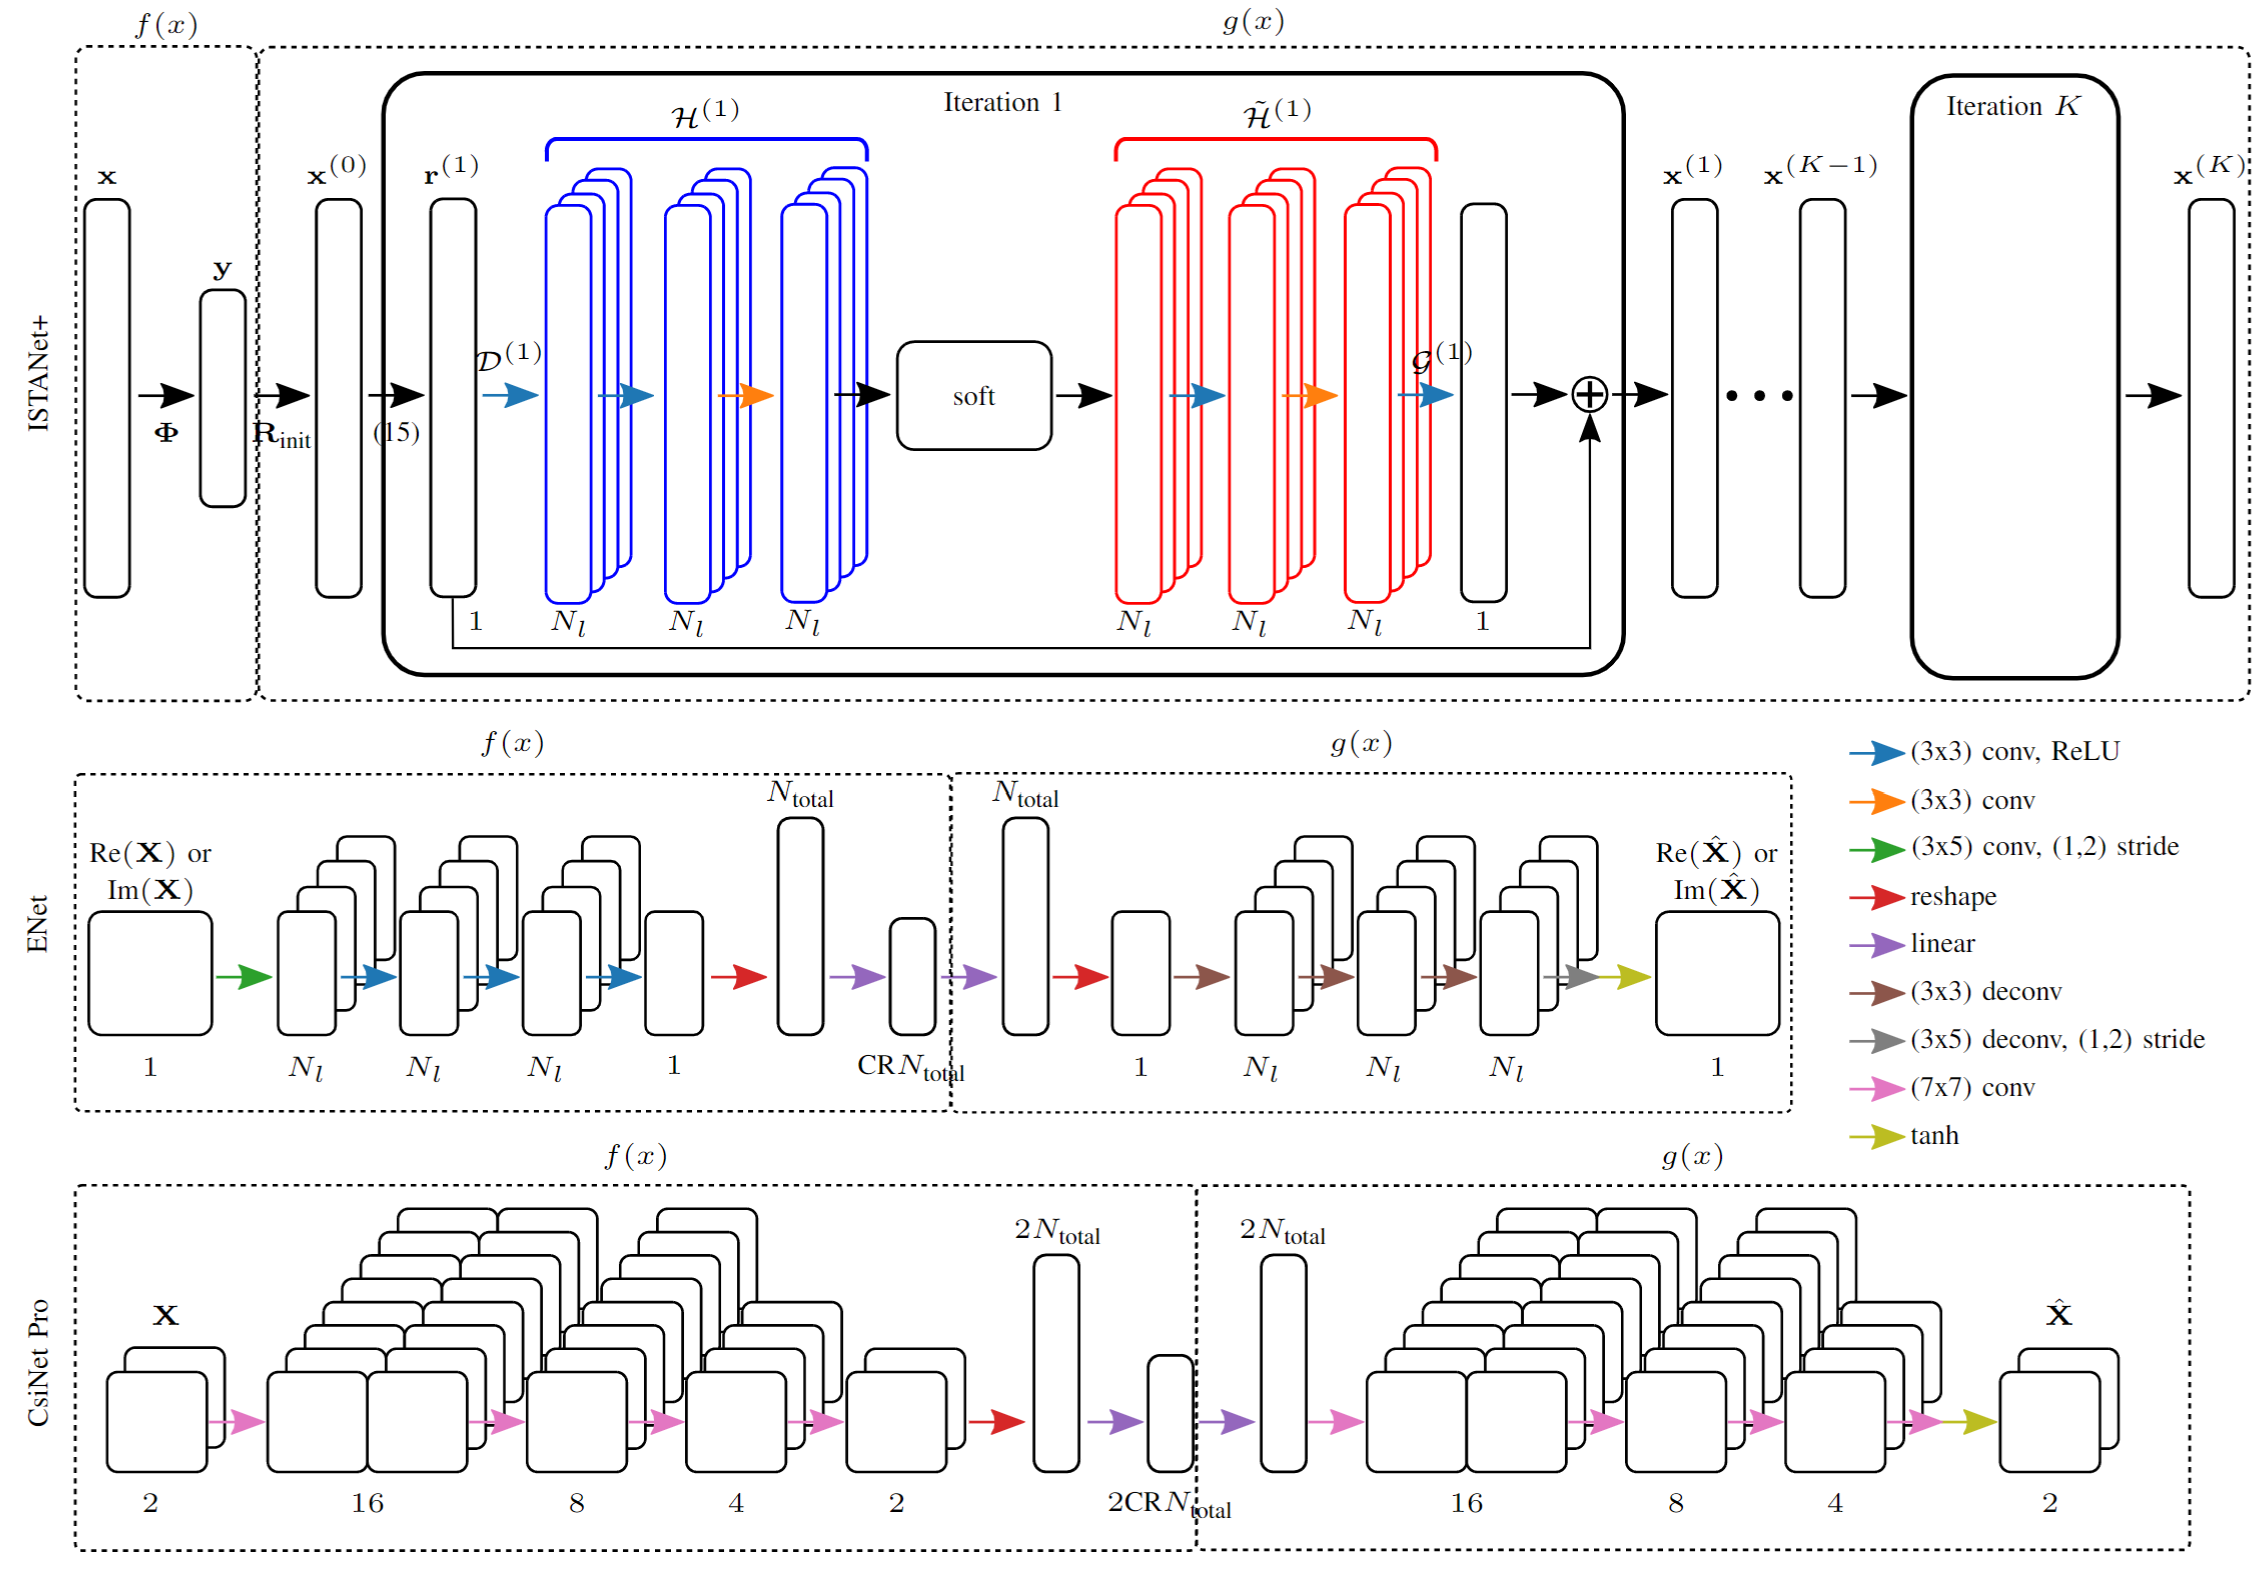
\includegraphics[width=\linewidth]{images/arch-comparison.png}
    % \input{figure/csinet_quant.pdf_tex}
    \caption{Compressive CSI estimation architectures used in this work. $f(x)$ denotes the encoder, and $g(x)$ denotes the decoder. $N_{\text{total}}=N_bN_t$ is the size of the real or imaginary channel. $N_l$ is the number of latent channels in a convolutional layer.}
    \label{fig:arch_compare}
\end{figure}

\subsection{Iterative Optimization Networks for CS-based CSI Feedback} \label{sec:iter-cs}

% In \cite{ref:zhang2018ista}, the authors emulate the iterations of the Iterative Shrinkage-Thresholding Algorithm (ISTA) as lightweight CNNs. They propose a network (ISTANet+) which utilizes skip connections in each iteration to learn the residual of the reconstructed image.
 
While CNN autoencoders have been dominant in CSI estimation, recent work from image processing has shown promise in using trainable CS algorithms based on CNNs\footnote{For an overview of conventional compressive sensing solutions as well as the original ISTA algorithm, see Appendix~\ref{appdx:compressed-sensing}}. These works treat iterative CS algorithms as sequential networks by ``unrolling'' them into discrete blocks \cite{ref:yang2016deep, ref:zhang2018ista}. Investigating unrolled CS algorithms for CSI estimation warrants consideration, as CS algorithms can have guaranteed convergence under mild sparsity conditions (in contrast with CNNs autoencoder approaches, which do not have such guarantees). Since CSI data exhibits sparsity in the delay domain, specifying an appropriate compressive sensing approach could provide appreciable performance gains in our differential CSI encoding architecture. 

To exploit the temporal coherence of the MIMO channel, we propose to construct a differential encoding network using an unrolled optimization network based on a trainable version of the iterative shrinkage-thresholding algorithm (ISTA), called ISTANet+ \cite{ref:zhang2018ista}. See the top of Figure~\ref{fig:arch_compare} for a diagram of ISTANet+. Denote measurement matrix for the ISTANet+ as 
\begin{align}
    \mathbf \Phi \in \mathbf{R}^{N_{\text{total}}\text{CR} \times N_{\text{total}}}.
\end{align}
For compressive sensing approaches, the measurement matrix is analogous to the `encoder' of autoencoder approaches, i.e., $f(x)=\mathbf\Phi x$. The `decoder' consists of $K$ iterations of the following update steps,
\begin{align}
    \mathbf{r}^{(k)} &= \mathbf{x}^{(k-1)}-\rho^{(k)}\mathbf{\Phi}^\top(\mathbf{\Phi}\mathbf x^{(k-1)}-\mathbf y) \label{eq:istanet-grad} \\
    % \mathbf x^{(k)} &= \tilde{\mathcal{F}}^{(k)}\left(\text{soft}\left(\mathcal{F}^{(k)}(\mathbf{r}^{(k)}), \theta^{(k)}\right)\right)
    \mathbf x^{(k)} &= \mathbf{r}^{(k)} + \mathcal{G}^{(k)}\left(\tilde{\mathcal{H}}^{(k)}\left(\text{soft}\left(\mathcal{H}^{(k)}(\mathcal{D}^{(k)}(\mathbf{r}^{(k)}), \theta^{(k)}\right)\right)\right) \label{eq:istanet-prox}
\end{align}
where $\mathbf y=\mathbf{\Phi} \mathbf x$, $\mathbf x^{(0)}=\mathbf{R}_{\text{init}}\mathbf{y}$, and $\mathbf R_{\text{init}}=\mathbf {XY}(\mathbf{YY}^\top)^{-1}$ is the initialization matrix for the training data matrix $\mathbf X = \left[\mathbf{x}_1, \mathbf{x}_2,\dots, \mathbf{x}_{N_{\text{train}}}\right]$ and the training measurement matrix $\mathbf Y = \left[\mathbf{y}_1, \mathbf{y}_2,\dots, \mathbf{y}_{N_{\text{train}}}\right]$. `soft($\cdot$)' denotes the soft threshold function,
\begin{align}
    \text{soft}(x, \theta) &= \text{sign}(x)\text{ReLU}(|x|-\theta). \label{eq:soft}
\end{align}
$\mathcal G^{(k)}, \mathcal D^{(k)},  \mathcal H^{(k)}, \tilde{\mathcal H}^{(k)}$ indicate trainable nonlinear mappings (in this case, CNNs), and $\mathcal H^{(k)}, \tilde{\mathcal H}^{(k)}$ are subject to the symmetry constraint $\mathcal H^{(k)}\circ \tilde{\mathcal H}^{(k)}=\mathbf I$\footnote{Where $\circ$ denotes the function composition, $(f \circ g)(x) = f(g(x))$}. The rectified linear unit (ReLU) is given as
\begin{align*}
    \text{ReLU}(x) &= 
        \begin{cases}
            x & x \geq 0 \\
            0 & x < 0
        \end{cases}
\end{align*}
In the proposed differential encoding scheme, we use an instance of ISTANet+ in the first timeslot, $t_1$, with a large compression ratio such that $\text{CR}_{t_1} \geq \text{CR}_{t_i}$ for all $i > 1$. This choice in compression ratio allows us to initialize the network with a high-quality estimate at the first timeslot. Notably, the training data matrix, $\mathbf X$, differs between timeslots. For the first timeslot, the data vectors $\mathbf{x}_i$ are vectorized versions of the CSI matrices,
\begin{align}
    \mathbf{x}_j &= \text{vec}\left(\mathbf{H}^{(j)}_{\tau,1}\right) \text{ for } j\in[N_{\text{train}}]. 
    \label{eq:t1_vec}
\end{align}
However, the data vectors for all other timeslots are vectorized versions of the error matrices,
\begin{align}
    \mathbf{x}_j &= \text{vec}\left(\bar{\mathbf{E}}^{(j)}_{i}\right) \text{ for } j\in[N_{\text{train}}]. 
    \label{eq:ti_vec}
\end{align}
Denote the parameters for ISTANet+ in the $t_i$-th timeslot as $\mathbf{\Theta}_{t_i}=\{\mathcal G^{(k)}, \mathcal D^{(k)},  \mathcal H^{(k)}, \tilde{\mathcal H}^{(k)}, \theta^{(k)}, \rho^{(k)}\}_{k=1}^{K}$. The loss function is a weighted sum of the MSE and the symmetry constraint, i.e.,
\begin{align}
    L(\mathbf{\Theta}_{t_i}) &= L_{\text{MSE}} + \alpha L_{\text{sym}} \\
    L_{\text{MSE}} &= \frac{1}{N_{\text{batch}}N_{\text{total}}}\sum_{i=1}^{N_{\text{batch}}}\|\mathbf{x}_i^{(K)}-\mathbf{x}_i\|_2^2 \\
    L_{\text{sym}} &= \frac{1}{N_{\text{batch}}N_{\text{total}}}\sum_{i=1}^{N_{\text{batch}}}\sum_{k=1}^{K} \|\tilde{\mathcal{H}}^{(k)}(\mathcal{H}^{(k)}(\mathbf{x}_i)) - \mathbf{x}_i)\|_2^2
\end{align}
where $N_{\text{total}}=N_bN_t$ is the size of the truncated CSI matrix, $K$ is the number of iterations in ISTANet+, and $N_{\text{batch}}$ is the batch size used during training. As denoted in equations (\ref{eq:t1_vec}) and (\ref{eq:ti_vec}), the vectors $\mathbf{x}_i$ depend on the timeslot.

\begin{figure}[!hbtp]
    \centering
    {
      \fontsize{8pt}{8pt}
      \def\svgwidth{1.0\linewidth}
      \input{./images/02_markov_ista_p2d.pdf_tex}
    }
    % \input{figure/csinet_quant.pdf_tex}
    \caption{Diagram of a CSI estimation network using compressed differential feedback based on the linear P2DE. First, downlink pilots are used to estimate a downsampled frequency domain CSI estimate, $\bar{\mathbf{H}}_t\in\mathbb{C}^{N_b \times M_f}$ where $M_f << N_f$ at the $t$-th timeslot. Then, the P2DE $\mathbf{Q}^\#_{N_t}$ of Algorithm~\ref{alg:p2d-diag} is applied to estimate $\tilde{\mathbf{H}}_t$. After P2DE, the learnable transforms $f_t(x)$ and $g_t(x)$ are used to compress and decode the feedback, respectively. For $t=1$, the encoder/decoder are applied directly to $\tilde{\mathbf{H}}_1$. In all subsequent timeslots ($t > 1$), the differential term $\mathbf{E}_t$ is compressed and fed back.}
    \label{fig:markov-p2d}
\end{figure}

\section{Results}
\label{sect:p2de-results}

\subsection{Accuracy of P2DE}

 We assess the accuracy of the P2DE under values of $M_f$ and $D$. Fig.~\ref{fig:outdoor_p2d_init} demonstrates the accuracy of the P2DE at the UE (i.e., before compression and feedback) for different frequency downsampling ratios. The P2DE achieves impressive accuracy even under aggressive values of $\text{DR}_f$ (e.g., better than $-30$dB at $\text{DR}_f=\frac 18$). Additionally, the effect of increasing the diagonal size, $D$, is apparent at larger compression ratios (i.e., $\text{CR} \geq \frac 18$), where the accuracy of the P2DE to a value as low as $-25$dB. For smaller compression ratios (i.e., $\text{CR} \leq \frac {1}{16}$), increasing $D$ has a marginal effect on the accuracy of the P2DE.

 \begin{figure}[!hbtp]
    \centering
    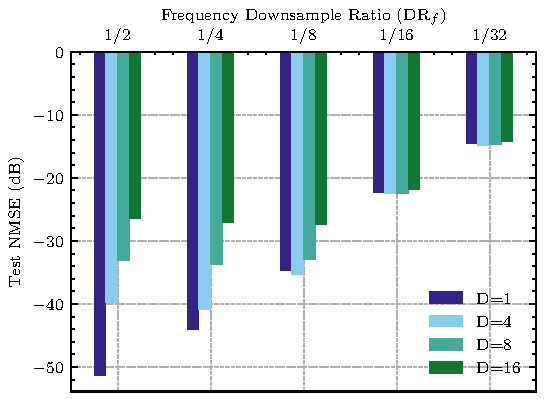
\includegraphics{./images/outdoor_p2d_diag.pdf}
    \caption{P2D estimation performance under different frequency downsampling ratios ($\text{DR}_f=\frac{M_f}{N_f}$) and diagonal dimensions ($D$) for the Outdoor COST2100 dataset. Downsampling is done along the frequency axis.}
    \label{fig:outdoor_p2d_init}
\end{figure}

We assess the accuracy of the P2DE assuming noise from pilot estimation. To simulate pilot estimation error, we use additive Gaussian noise,
\begin{align*}
    \hat{\mathbf{H}}_d &= \mathbf{H}_d + \mathbf{N}_d
\end{align*}
where the elements of $\mathbf{N}_d$, $\mathbf{N}_d(i,j) \sim \mathcal{N}(0, \sigma^2)$ for $i \in \left[1,2,\dots, N_b\right], j \in \left[1,2,\dots, M_f\right]$. To achieve different SNR values for $\hat{\mathbf{H}}_d$, we simply vary the noise variance $\sigma^2$, and we use the P2DE at different pilot estimation noise levels. Figure~\ref{fig:snr_sweep} shows the accuracy of the P2DE for different values of $\sigma^2$.

In addition to varying the pilots estimation SNR, we also showcase the effect of varying $\delta$ (i.e., the ODIR parameter as described in Appendix~\ref{appdx:odir}). We observe that $\delta$ helps the P2DE achieve better performance under both low-noise and noisy conditions, i.e.,

\begin{itemize}
    \item \textbf{Low-noise condition (SNR $\mathbf{=-20}$ dB)}: The P2DE goes from $-8$ dB to $-22$ dB for $\delta=0$ and $\delta=0.5$, respectively.
    \item \textbf{Noisy condition (SNR $\mathbf{\geq -10}$ dB)}: The P2DE goes from $-9$ dB to $-30$ dB for $\delta=0$ and $\delta=0.5$, respectively.
\end{itemize}

\begin{figure}[!hbtp]
    \centering
    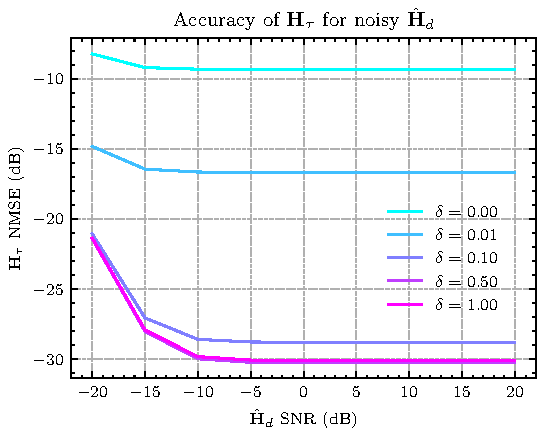
\includegraphics{outdoor_snr_sweep_delta_D4_sz32.pdf}
    \caption{Accuracy of P2DE output, $\mathbf{H}_{\tau}$, assuming noisy pilots, $\hat{\mathbf{H}}_d$. Additive Gaussian noise is used to model the error inherent in pilot estimation. Here, $D=4, \text{DR}_f=\frac{1}{32}$.}
    \label{fig:snr_sweep}
\end{figure}

\subsection{P2DE Compression Network Comparison}

Having assessed the initial accuracy of the P2DE at the UE, we now apply a deep learning network to compress the output of the P2DE. Figure~\ref{fig:outdoor_drcr_sweep} demonstrates the accuracy of ISTANet+ \cite{ref:zhang2018ista} for multiple compression ratios (CR) using the P2DE as its input. For progressively smaller compression ratios, the accuracy of ISTANet+ remains stable until $\text{DR}_f=\frac{1}{32}$, at which point the network's performance degrades.

\begin{figure}[!hbtp]
    \centering
    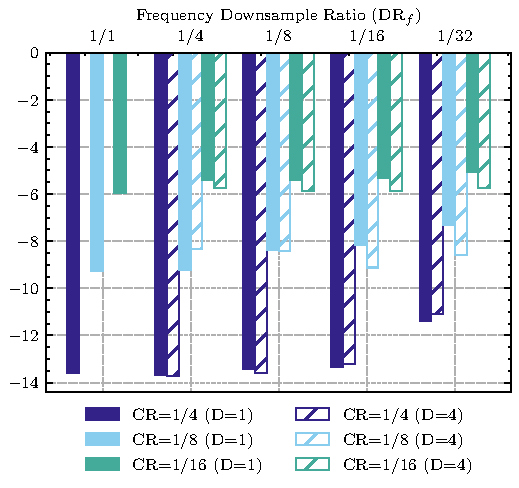
\includegraphics{./images/outdoor_drcr_D_sweep.pdf}
    \caption{Performance of ISTANet+ for multiple compression ratios using P2D estimates with different downsampling ratios ($\text{DR}_f=\frac{M_f}{N_f}$) for the Outdoor COST2100 dataset. Non-diagonal pattern ($D=1$) is compared with a diagonal pattern of size $D=4$. Performance for $\text{DR}_f=1/1$, $D=4$ is omitted since it is equivalent to the $\text{DR}_f=1, D=1$ case.}
    \label{fig:outdoor_drcr_sweep}
\end{figure}

In addition to ISTANet+, we assess the accuracy deep CNN autoencoders using P2DE as an input. Figure~\ref{fig:outdoor_net_ablation} shows the accuracy of ISTANet+ compared to ENet \cite{ref:Sun2021ENet} and SphNet \cite{ref:liu2020sphnet}. The performance of ISTANet+ is better than both ENet and SphNet at larger compression ratios ($\text{CR}\in [\frac 14, \frac 18]$), and the performance of ISTANet+ and ENet is comparable at $\text{CR}=\frac {1}{16}$.

\begin{figure}[!hbtp]
    \centering
    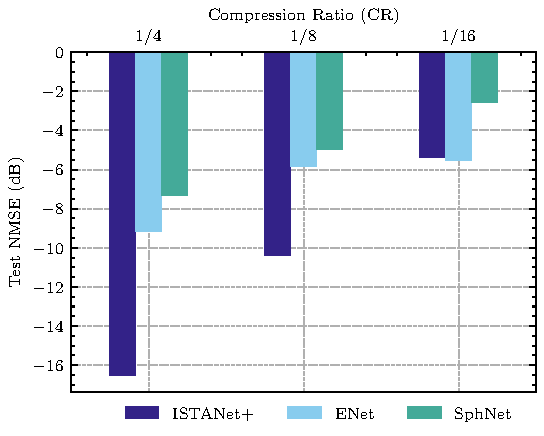
\includegraphics{outdoor_net_compare.pdf}
    \caption{Performance comparison for different feedback compression networks using P2D estimates ($\text{DF}_f=1/16, D=4$) for Outdoor COST2100 dataset. For all tested networks, we use $N_{\text{phase}}=4$, resulting in an augmented training set with $80$k samples.}
    \label{fig:outdoor_net_ablation}
\end{figure}

To assess the accuracy of these networks under quantization, we also conduct an experiment where the latent feedback elements are subjected to $\mu$-law companding and uniform quantization (as described in Section~\ref{sec:markov-results}). We present these results in Figure~\ref{fig:net_quant}.

\begin{figure}[!hbtp]
    \centering
    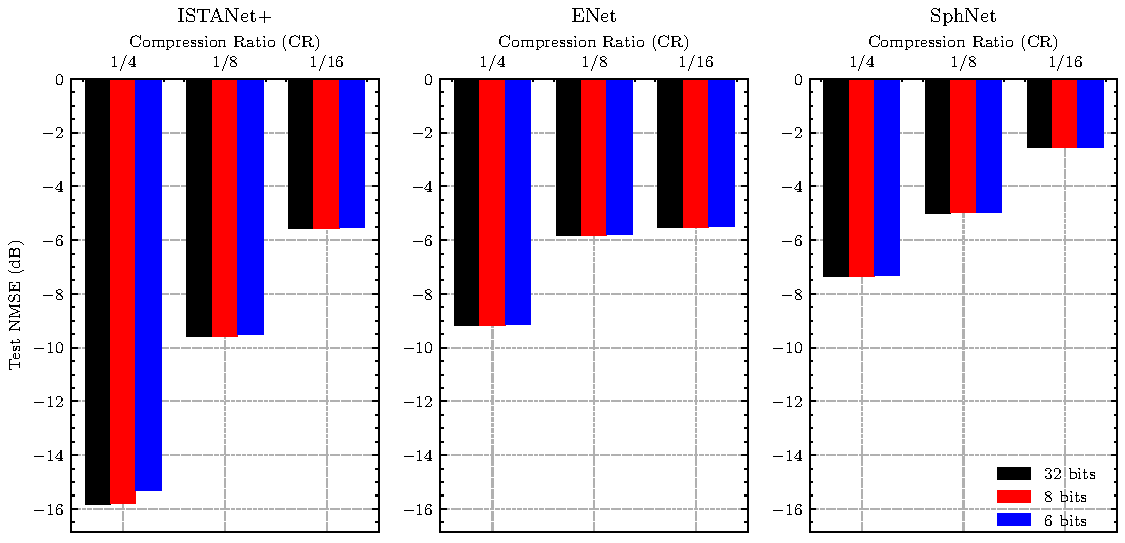
\includegraphics[width=\linewidth]{./images/outdoor_net_quant.pdf}
    \caption{Tested networks where feedback is subject to $\mu$-law companding ($\mu=255$) and uniform quantization for different numbers of quantization bits. P2DE parameters are $D=4, \text{DR}_f=\frac{1}{16}$.}
    \label{fig:net_quant}
\end{figure}

\subsection{Heterogeneous Differential Encoding Networks}

Figure~\ref{fig:markov-p2d-results} shows the performance of the proposed heterogeneous differential encoding networks compared to homogeneous networks. We observe that ENet provides worse initial performance than ISTANet+ (i.e., at $t_1$) but provides a more improvement in accuracy than ISTANet+ in subsequent timeslots (i.e., at $t_2, t_3, \dots$). Based on this observation, we expect the best network configuration to be the heterogeneous network, MN-IE. Figure~\ref{fig:markov-p2d-results} supports this reasoning, as MN-IE achieves better asymptotic performance (i.e., as $i$ for $t_i$ increases) than MN-I.

\begin{figure}[!hbtp]
    \centering
    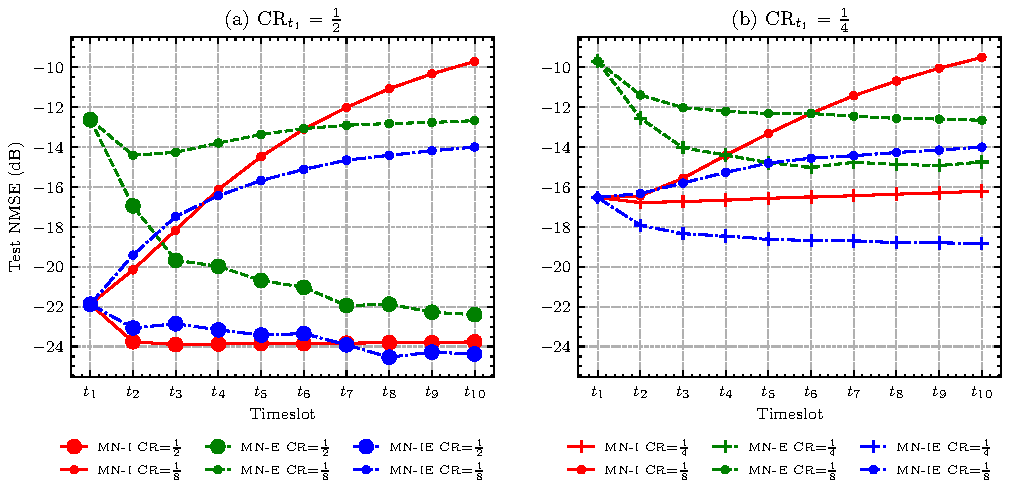
\includegraphics{outdoor_markov_sweep_v2.pdf}
    \caption{Compressive CSI estimation using differential encoding and  linear P2D estimator ($M_f=128, \text{DR}_f=\frac{1}{8}, D=4$). MarkovNet-ISTA (MN-I), MarkovNet-ENet (MN-E), and MarkovNet-ISTA-ENet (MN-IE) are tested using two different compression ratios in the first timeslot, $\text{CR}_{t_1}\in\left[\frac{1}{2},\frac{1}{4}\right]$.}
    \label{fig:markov-p2d-results}
\end{figure}

\subsection{Computational Complexity}

We assess the computational complexity (as defined in Chapter~\ref{chap:sph_norm}, Section~\ref{sect:dl_overview}) of the network architectures tested in this work. While ISTANet+ has superior accuracy compared to the autoencoder networks, we observe that its computational complexity is much higher. This discrepancy in complexity further motivates the heterogeneous network architecture of MN-IE. While MN-I uses $T$ copies of ISTANet+, MN-IE uses one copy of ISTANet+ to provide an initial estimate and $T-1$ copies of ENet to compress the differential term.

\begin{table}[htb]
\centering
\caption{Computational complexity of networks used in this work. \textbf{Bold face} in a column indicates lowest value for given compression ratio. ``CR" $=$ compression ratio, ``Enc" $=$ encoder, ``Dec" $=$ decoder. FLOPs indicate computation during inference (i.e., not training/back-propagation).}
\label{tab:net-complexity} 

\begin{tabular}{|cc|cccc|cc|}
\hline
\multicolumn{2}{|c|}{\multirow{2}{*}{}}                    & \multicolumn{4}{c|}{Parameters (M)}                                                                                          & \multicolumn{2}{c|}{\multirow{2}{*}{FLOPs (M)}}     \\ \cline{3-6}
\multicolumn{2}{|c|}{}                                     & \multicolumn{2}{c|}{Trainable}                                          & \multicolumn{2}{c|}{All}                           & \multicolumn{2}{c|}{}                               \\ \hline
\multicolumn{1}{|c|}{}                            & CR     & \multicolumn{1}{c|}{Enc}           & \multicolumn{1}{c|}{Dec}           & \multicolumn{1}{c|}{Enc}           & Dec           & \multicolumn{1}{c|}{Enc}           & Dec            \\ \hline
\multicolumn{1}{|c|}{\multirow{4}{*}{ISTANet+}}    & $1/2$  & \multicolumn{1}{c|}{\textbf{0.00}} & \multicolumn{1}{c|}{\textbf{0.34}} & \multicolumn{1}{c|}{2.10}          & 4.54          & \multicolumn{1}{c|}{\textbf{2.10}} & 393.78         \\ \cline{2-8} 
\multicolumn{1}{|c|}{}                            & $1/4$  & \multicolumn{1}{c|}{\textbf{0.00}} & \multicolumn{1}{c|}{0.34}          & \multicolumn{1}{c|}{1.05}          & 2.44          & \multicolumn{1}{c|}{\textbf{1.05}} & 373.85         \\ \cline{2-8} 
\multicolumn{1}{|c|}{}                            & $1/8$  & \multicolumn{1}{c|}{\textbf{0.00}} & \multicolumn{1}{c|}{0.34}          & \multicolumn{1}{c|}{0.52}          & 1.39          & \multicolumn{1}{c|}{\textbf{0.52}} & 363.89         \\ \cline{2-8} 
\multicolumn{1}{|c|}{}                            & $1/16$ & \multicolumn{1}{c|}{\textbf{0.00}} & \multicolumn{1}{c|}{0.34}          & \multicolumn{1}{c|}{0.26}          & 0.87          & \multicolumn{1}{c|}{\textbf{0.26}} & 358.91         \\ \hline
\multicolumn{1}{|c|}{\multirow{4}{*}{ENet}}       & $1/2$  & \multicolumn{1}{c|}{0.55}          & \multicolumn{1}{c|}{0.55}          & \multicolumn{1}{c|}{\textbf{0.55}} & \textbf{0.55} & \multicolumn{1}{c|}{29.98}         & 29.70          \\ \cline{2-8} 
\multicolumn{1}{|c|}{}                            & $1/4$  & \multicolumn{1}{c|}{0.29}          & \multicolumn{1}{c|}{\textbf{0.29}} & \multicolumn{1}{c|}{\textbf{0.29}} & \textbf{0.29} & \multicolumn{1}{c|}{29.46}         & 29.18          \\ \cline{2-8} 
\multicolumn{1}{|c|}{}                            & $1/8$  & \multicolumn{1}{c|}{0.16}          & \multicolumn{1}{c|}{\textbf{0.16}} & \multicolumn{1}{c|}{\textbf{0.16}} & \textbf{0.16} & \multicolumn{1}{c|}{29.20}         & 28.92          \\ \cline{2-8} 
\multicolumn{1}{|c|}{}                            & $1/16$ & \multicolumn{1}{c|}{0.09}          & \multicolumn{1}{c|}{\textbf{0.09}} & \multicolumn{1}{c|}{\textbf{0.09}} & \textbf{0.09} & \multicolumn{1}{c|}{29.07}         & 28.79          \\ \hline
\multicolumn{1}{|c|}{\multirow{4}{*}{CsiNet Pro}} & $1/2$  & \multicolumn{1}{c|}{1.06}          & \multicolumn{1}{c|}{1.06}          & \multicolumn{1}{c|}{1.06}          & 1.06          & \multicolumn{1}{c|}{12.16}         & \textbf{12.16} \\ \cline{2-8} 
\multicolumn{1}{|c|}{}                            & $1/4$  & \multicolumn{1}{c|}{0.53}          & \multicolumn{1}{c|}{0.53}          & \multicolumn{1}{c|}{0.53}          & 0.53          & \multicolumn{1}{c|}{11.11}         & \textbf{11.11} \\ \cline{2-8} 
\multicolumn{1}{|c|}{}                            & $1/8$  & \multicolumn{1}{c|}{0.27}          & \multicolumn{1}{c|}{0.27}          & \multicolumn{1}{c|}{0.27}          & 0.27          & \multicolumn{1}{c|}{10.59}         & \textbf{10.59} \\ \cline{2-8} 
\multicolumn{1}{|c|}{}                            & $1/16$ & \multicolumn{1}{c|}{0.14}          & \multicolumn{1}{c|}{0.14}          & \multicolumn{1}{c|}{0.14}          & 0.14          & \multicolumn{1}{c|}{10.33}         & \textbf{10.33} \\ \hline
\end{tabular}
\end{table}
